\documentclass[conference]{IEEEtran}
\IEEEoverridecommandlockouts

\usepackage{cite}
\usepackage{amsmath,amssymb,amsfonts}
\usepackage{algorithmic}
\usepackage{graphicx}
\usepackage{textcomp}
\usepackage{xcolor}
\usepackage{booktabs}
\usepackage{tabularx}
\usepackage{balance}
\usepackage{url}
\usepackage{microtype}

% Relax float placement parameters to keep figures with text and prevent orphan float pages
\renewcommand{\topfraction}{0.95}
\renewcommand{\bottomfraction}{0.95}
\renewcommand{\textfraction}{0.05}
\renewcommand{\floatpagefraction}{0.85}
\renewcommand{\dbltopfraction}{0.95}
\renewcommand{\dblfloatpagefraction}{0.85}

\graphicspath{{figures/}}

\def\BibTeX{{\rm B\kern-.05em{\sc i\kern-.025em b}\kern-.08em
    T\kern-.1667em\lower.7ex\hbox{E}\kern-.125emX}}

\begin{document}

\title{A Real-Time Adaptive Digital Communication System for Intelligent Line-Code Selection Under Simulated Underwater Acoustic Channel Conditions}

% Single-column author block: all author details in a single centered column
\author{
    \IEEEauthorblockN{Ekanshi Yadav (24BEC0655), \quad Shailesh A (24BEC0665), \quad Sheshadri Muthusamy (24BEC0250)}
    \IEEEauthorblockA{\textit{School of Electronics Engineering (SENSE), Vellore Institute of Technology}, Vellore, Tamil Nadu, India \\
    Email: ekanshi.yadav2024@vitstudent.ac.in, \quad shailesh.2024@vitstudent.ac.in, \quad sheshadri.m2024@vitstudent.ac.in}
}

\maketitle

\begin{abstract}
Underwater acoustic channels present severe transmission impairments, including frequency-dependent Thorp absorption, three-path surface/bottom multipath reflections, and carrier Doppler shifts caused by relative vehicle motion. Consequently, relying on a single static line code cannot satisfy diverse operational demands. In this work, we propose and implement \textbf{SignalForge}, an intelligent hybrid communication framework that evaluates six baseband line codes: Non-Return-to-Zero Level (NRZ-L), Non-Return-to-Zero Inverted (NRZ-I), Return-to-Zero (RZ), Manchester, Alternate Mark Inversion (AMI), and Differential Manchester. To solve the computational latency problem of brute-force physical simulation ($80$--$200$~ms per evaluation), we introduce a Dual-Engine architecture: an offline high-fidelity acoustic channel simulator that establishes physical ground truth, paired with a lightweight, edge-deployable $9$-dimensional $k$-nearest-neighbor ($k$-NN, $k=5$) classifier that predicts the optimal line code in under $0.5$~ms ($\approx 360\times$ acceleration). The model supports both a multi-attribute Simple Additive Weighting (SAW) utility function and a minimum-Bit Error Rate (BER) oracle. Experimental sweeps validate that while NRZ-L and AMI minimize bandwidth occupancy ($910$~Hz and $1045$~Hz), Manchester and Differential Manchester ensure continuous clock synchronization ($1.5$ transitions/bit) and robust bit recovery under low SNR and multipath. The system is deployed via a standalone, zero-dependency web dashboard with automated MATLAB script generation for complete scientific reproducibility.
\end{abstract}

\begin{IEEEkeywords}
Digital Communication Systems, Line Coding, Underwater Acoustic Channel, Adaptive Decision Engine, $k$-Nearest Neighbor, Simple Additive Weighting, Machine Learning.
\end{IEEEkeywords}

\section{Introduction}
Underwater acoustic communication (UWAC) is fundamentally constrained by physical propagation limitations. Acoustic absorption increases sharply with carrier frequency and distance, multi-path boundary reflections produce severe frequency-selective fading, and vehicular platform drifts induce pronounced Doppler spreading~\cite{stojanovic2009underwater}.

Before baseband waveforms modulate an acoustic carrier frequency, digital line coding defines voltage representation, occupied spectral density, direct-current (DC) content, and self-clocking transition density~\cite{proakis2008digital}. However, these physical attributes impose strict trade-offs:
\begin{itemize}
    \item \textbf{Bandwidth vs. Synchronization:} Manchester coding guarantees mid-bit transitions for clock recovery, but doubles bandwidth compared to NRZ-L.
    \item \textbf{DC Balance vs. Run-Length Invariance:} Alternate Mark Inversion (AMI) eliminates DC drift across transformer-coupled hydrophones, but long sequences of zeros starve timing recovery loops.
    \item \textbf{Polarity vs. Error Propagation:} Differential schemes (NRZ-I, Differential Manchester) resolve $180^\circ$ phase ambiguities, but channel bit errors can corrupt adjacent symbols.
\end{itemize}
Because ocean conditions fluctuate with tides, range, and current velocity, no single baseband scheme is universally optimal. While contemporary research adapts carrier modulation or forward error correction~\cite{li2024reinforcement, chen2025optimal, jing2024adaptive, survey2026amc, adaptive2023profile, fan2021adaptive, kadali2025ai}, dynamic selection among baseband line codes under multi-attribute acoustic metrics remains largely unexplored.

\subsection{Research Objectives}
This project accomplishes five engineering objectives:
\begin{enumerate}
    \item \textbf{Multi-Scheme Implementation:} Synthesize six digital line codes on uniform test bit sequences.
    \item \textbf{Acoustic Channel Modeling:} Convolve waveforms through Thorp frequency attenuation, multipath spreading, and Doppler drift.
    \item \textbf{Physical Metric Extraction:} Quantify empirical Bit Error Rate (BER), $90\%$ power spectral containment, DC balance, and clock transition density.
    \item \textbf{Dual-Engine ML Selector:} Develop a standardized $9$-D $k$-NN classifier offering sub-millisecond adaptive selection under both multi-attribute (SAW) and minimum-BER objectives.
    \item \textbf{Zero-Dependency Deployment:} Implement a standalone, interactive dashboard with dynamic MATLAB code generation.
\end{enumerate}

\section{Related Work and Literature Review}
Adaptive communication in underwater acoustics has predominantly focused on carrier-level Adaptive Modulation and Coding (AMC). Table~\ref{tab:lit_review} provides a comparative summary of relevant contemporary studies.

\begin{table*}[!t]
\centering
\caption{Comparative Summary of Related Underwater Acoustic Communication Works}
\label{tab:lit_review}
\begin{tabularx}{\textwidth}{@{}l c p{3.2cm} X X@{}}
\toprule
\textbf{Reference} & \textbf{Year} & \textbf{Primary Approach} & \textbf{Key Capabilities} & \textbf{Relevance / Distinction to SignalForge} \\
\midrule
Li \textit{et al.}~\cite{li2024reinforcement} & 2024 & Reinforcement Learning (Q-learning) & Automated carrier switching across FH-BFSK, ASK, PSK, OFDM & Carrier modulation switching; does not address baseband line-code pulse formats. \\
Chen \textit{et al.}~\cite{chen2025optimal} & 2025 & Random Forest Classifier & Adaptive coding-and-modulation mode selection via SNR and channel impulse response & Demonstrates ML classification on acoustic features; focus is convolutional channel codes. \\
Jing \textit{et al.}~\cite{jing2024adaptive} & 2024 & CNN with Meta-Learning & AMC for underwater OTFS modulation across rapid channel variations & Proves value of fast adaptation; high neural complexity requires GPU inference. \\
Zhang \textit{et al.}~\cite{survey2026amc} & 2026 & Comprehensive Survey \& Benchmark & Evaluation of classical, ML, and RL-based AMC algorithms & Establishes acoustic benchmarks and validation metrics for adaptive link design. \\
Kim \textit{et al.}~\cite{adaptive2023profile} & 2023 & Deep Reinforcement Learning & Modem communication profile switching in varying ocean environments & Operates on discrete vendor modem presets rather than fundamental pulse representations. \\
Fan \& Wang~\cite{fan2021adaptive} & 2021 & DDPG with Gumbel-Softmax & Multimodal switching between FSK, single-carrier, and multicarrier blocks & Optimizes energy vs. spectral efficiency; does not optimize timing or DC balance. \\
Kadali \textit{et al.}~\cite{kadali2025ai} & 2025 & Decision Trees \& Random Forests & Cognitive modulation adaptation from environmental ocean telemetry & Uses environmental inputs ($T$, $S$, depth); validates feature-based edge decision making. \\
\midrule
\textbf{This Work (SignalForge)} & \textbf{2026} & \textbf{Hybrid Dual-Engine + 9-D $k$-NN} & \textbf{Real-time adaptation across 6 baseband line codes with SAW / Oracle objectives ($< 0.5$~ms)} & \textbf{First unified multi-criteria line-code selector optimizing BER, bandwidth, DC offset, and clock sync.} \\
\bottomrule
\end{tabularx}
\end{table*}

Existing literature establishes the viability of ML-based channel adaptation, but focuses on carrier schemes (PSK/QAM/OFDM) rather than the physical pulse format. SignalForge addresses this gap by selecting the baseband line code using an explicit multi-attribute framework.

\section{Theoretical Background}

\subsection{Line Coding Formats}
The framework evaluates six candidate schemes:
\begin{itemize}
    \item \textbf{NRZ-L:} Bit $1$ maps to $+V$ and bit $0$ to $-V$. Requires minimal bandwidth ($B_{90} \approx 910$~Hz at $1$~kbit/s), but suffers from DC baseline wander and loses clock sync during long runs of identical bits.
    \item \textbf{NRZ-I:} Signal level toggles at the start of bit $1$ and remains constant for bit $0$. Differential encoding provides polarity invariance, though single-bit errors propagate to double errors.
    \item \textbf{RZ:} A unipolar pulse occupies $+V$ for the first half of bit $1$ and returns to $0$~V; bit $0$ remains $0$~V. Introduces guaranteed edges on ones, but incurs non-zero DC bias ($+0.25 V$) and increased spectral spread ($B_{90} \approx 1850$~Hz).
    \item \textbf{Manchester:} Bit $1$ transitions from $-V$ to $+V$ at mid-bit; bit $0$ transitions from $+V$ to $-V$. Guaranteed transition in every bit guarantees clock synchronization with zero DC offset, at the cost of wider bandwidth ($B_{90} \approx 2820$~Hz).
    \item \textbf{AMI:} Bit $0$ is $0$~V, while successive $1$s alternate between $+V$ and $-V$. Strictly DC-free ($0.000$~V offset) and spectrally compact ($B_{90} \approx 1045$~Hz), but long sequences of zeros produce no transitions.
    \item \textbf{Differential Manchester:} A mid-bit transition always occurs; a transition at the start of the bit encodes $0$, while absence of an initial transition encodes $1$. Combines polarity invariance with continuous clock synchronization ($B_{90} \approx 2840$~Hz).
\end{itemize}

\subsection{Physical Evaluation Metrics}
Performance is quantified via four metrics:
\begin{enumerate}
    \item \textbf{Bit Error Rate (BER):} 
    \begin{equation}
        \text{BER} = \frac{N_{\text{err}}}{N_{\text{bits}}}
    \end{equation}
    where $N_{\text{err}}$ is the count of misdecoded bits over $N_{\text{bits}}$ transmitted bits.
    \item \textbf{$90\%$ Power Spectral Bandwidth ($B_{90}$):}
    \begin{equation}
        \int_{0}^{B_{90}} S(f) \, df = 0.90 \int_{0}^{\infty} S(f) \, df
    \end{equation}
    where $S(f)$ is the power spectral density estimated via periodogram.
    \item \textbf{DC Balance Metric ($M_{\text{DC}} \in [0, 1]$):}
    \begin{equation}
        M_{\text{DC}} = 1 - \frac{|\mu_v|}{V_{\text{peak}}}
    \end{equation}
    where $\mu_v$ is the mean waveform voltage and $V_{\text{peak}}$ is the peak amplitude. An ideal DC-free code yields $M_{\text{DC}} = 1.0$.
    \item \textbf{Clock Transition Density ($T_{\text{clk}}$):}
    \begin{equation}
        T_{\text{clk}} = \frac{N_{\text{edges}}}{N_{\text{bits}}}
    \end{equation}
    measuring the average number of voltage transitions per bit available for receiver phase-locked loop (PLL) tracking.
\end{enumerate}

Table~\ref{tab:code_characteristics} summarizes the measured baseline characteristics for each scheme.

\begin{table}[!htbp]
\centering
\caption{Baseline Physical Characteristics Across Candidate Line Codes}
\label{tab:code_characteristics}
\begin{tabular}{@{}l c c c c@{}}
\toprule
\textbf{Line Code} & \textbf{Levels} & \textbf{DC Balance} & \textbf{$B_{90}$ (Hz)} & \textbf{Transitions/Bit} \\
\midrule
NRZ-L & $2$ ($\pm 1$) & $0.965$ & $910$ & $0.49$ \\
NRZ-I & $2$ ($\pm 1$) & $0.990$ & $915$ & $0.51$ \\
RZ & $2$ ($0, +1$) & $0.000$ & $1850$ & $1.00$ \\
Manchester & $2$ ($\pm 1$) & $1.000$ & $2820$ & $1.50$ \\
AMI & $3$ ($0, \pm 1$) & $1.000$ & $1045$ & $0.76$ \\
Diff. Manchester & $2$ ($\pm 1$) & $1.000$ & $2840$ & $1.48$ \\
\bottomrule
\end{tabular}
\end{table}

\section{System Architecture and Problem Formulation}

\begin{figure*}[!t]
\centering
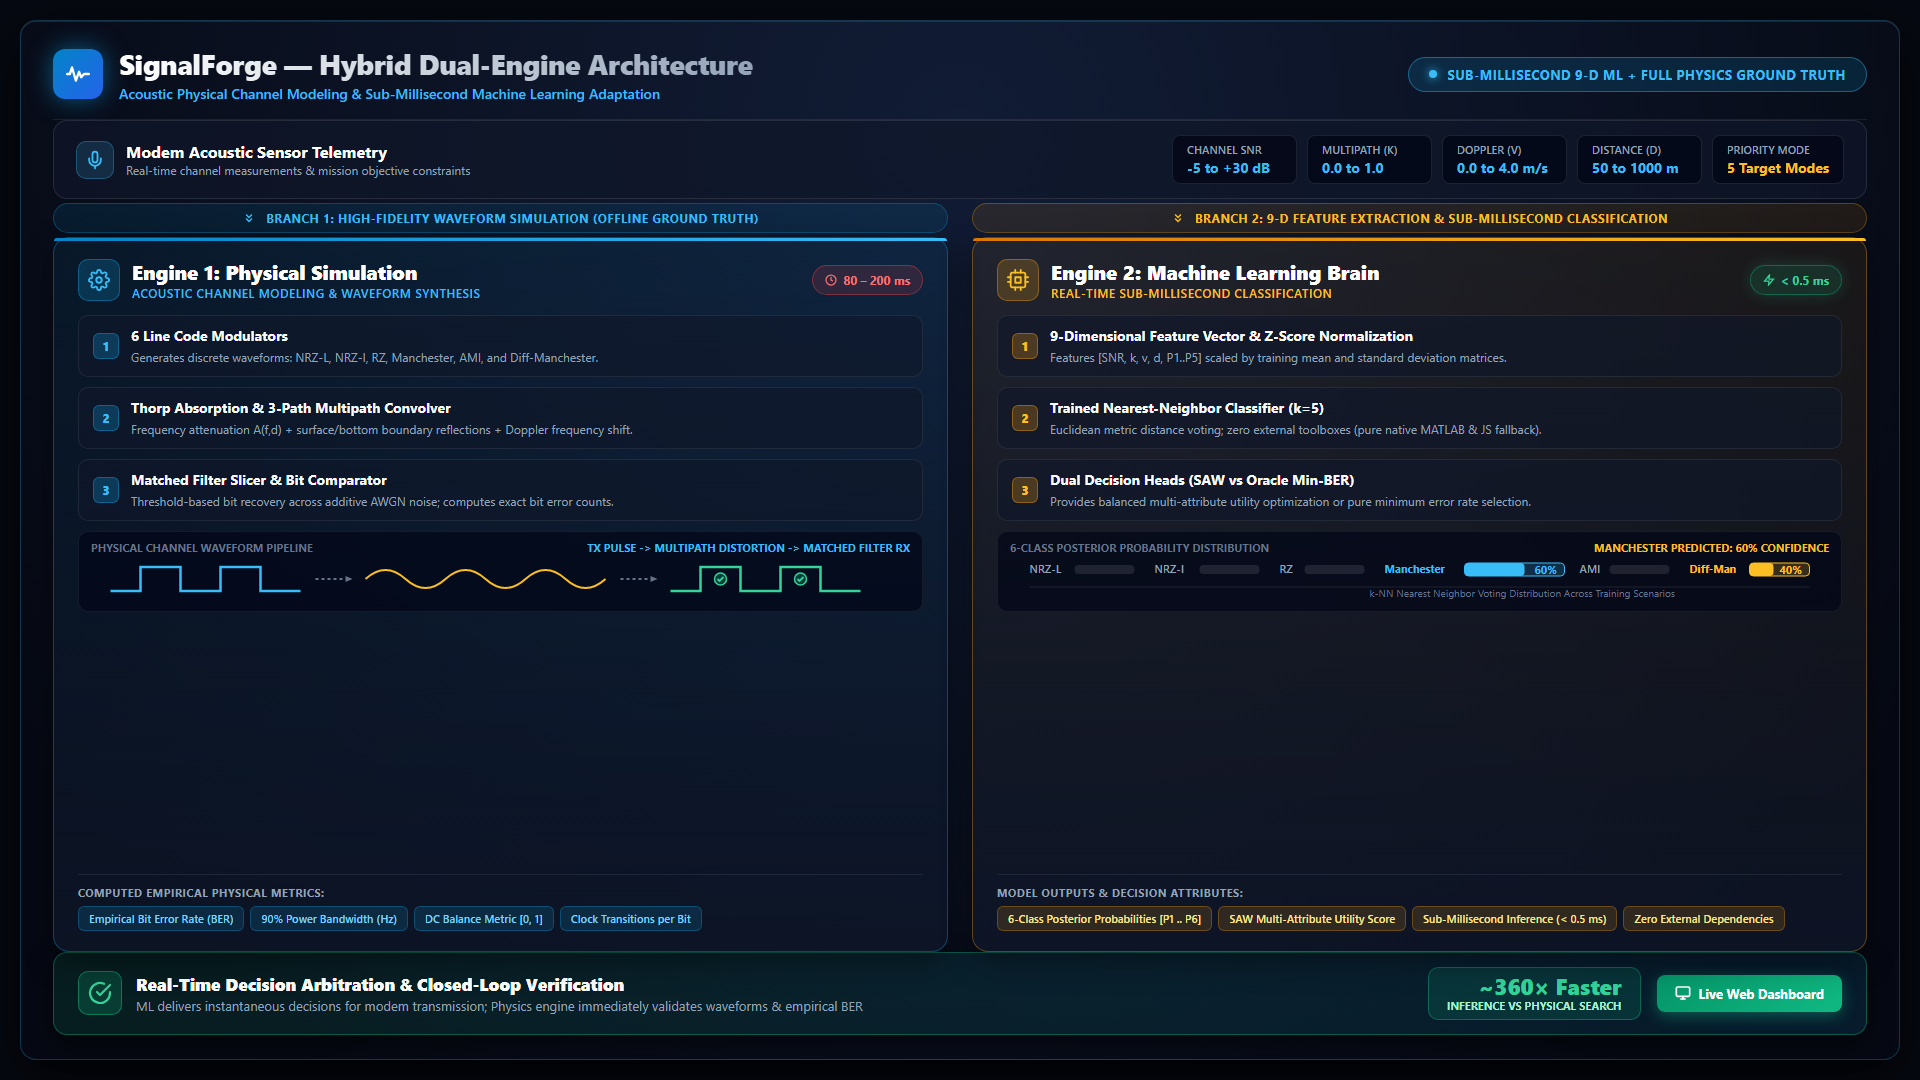
\includegraphics[width=0.88\textwidth,height=5.0cm,keepaspectratio]{fig1_architecture.png}
\caption{SignalForge Dual-Engine Architecture. Engine~1 performs physical acoustic waveform simulation ($80$--$200$~ms) to establish ground truth. Engine~2 utilizes a standardized $9$-D $k$-NN classifier ($< 0.5$~ms) for real-time edge adaptation, feeding an interactive verification dashboard.}
\label{fig:arch}
\end{figure*}

Fig.~\ref{fig:arch} illustrates the SignalForge Dual-Engine architecture. The system decouples slow physical simulation from real-time transmission adaptation.

Let $\mathcal{C} = \{\text{NRZ-L}, \text{NRZ-I}, \text{RZ}, \text{Manchester}, \text{AMI}, \text{Diff-Man}\}$ be the candidate set. The operating channel state is defined by the parameter vector:
\begin{equation}
    \boldsymbol{\theta} = [\text{SNR}, k, v, d]^T
\end{equation}
where $\text{SNR} \in [-5, 30]$~dB, multipath coefficient $k \in [0, 1]$, Doppler velocity $v \in [0, 4]$~m/s, and range $d \in [50, 1000]$~m.

The decision engine supports two distinct optimization heads:
\begin{enumerate}
    \item \textbf{Multi-Attribute SAW Head ($c_{\text{SAW}}^*$):}
    \begin{equation}
        c_{\text{SAW}}^* = \arg\max_{c \in \mathcal{C}} U(c \mid \boldsymbol{\theta}, \mathbf{p})
    \end{equation}
    where $U(c)$ is the Simple Additive Weighting utility function under priority vector $\mathbf{p}$.
    \item \textbf{Minimum-BER Oracle Head ($c_{\text{oracle}}^*$):}
    \begin{equation}
        c_{\text{oracle}}^* = \arg\min_{c \in \mathcal{C}} \text{BER}(c \mid \boldsymbol{\theta})
    \end{equation}
\end{enumerate}

\section{Proposed Adaptive Selection Framework}

\subsection{Engine 1: Physical Simulation Model}
Engine~1 establishes empirical ground truth through four sequential physical stages:
\begin{enumerate}
    \item \textbf{Thorp Absorption Loss:} Transmission loss $A(f, d)$ is computed using the empirical Thorp model~\cite{thorp1967analytic}:
    \begin{equation}
        \alpha(f) = \frac{0.11 f^2}{1 + f^2} + \frac{44 f^2}{4100 + f^2} + 2.75 \times 10^{-4} f^2 + 0.003
    \end{equation}
    for acoustic frequency $f$ in kHz and attenuation $\alpha(f)$ in dB/km. Range attenuation follows spherical geometric spreading $TL = 20 \log_{10}(d) + \alpha(f) d \times 10^{-3}$.
    \item \textbf{Three-Path Multipath Convolution:} Surface and seabed reflections are modeled via a discrete channel impulse response:
    \begin{equation}
        r(t) = s(t) + k a_1 s(t - \tau_1) + k a_2 s(t - \tau_2) + n(t)
    \end{equation}
    where delay spread $\tau_1, \tau_2 \le 4$~ms, $k \in [0, 1]$ scales reflection strength, and $a_1, a_2$ model boundary reflection losses.
    \item \textbf{Doppler Shift:} At carrier frequency $f_c = 5$~kHz and speed of sound $c = 1500$~m/s, relative platform velocity $v$ produces a carrier frequency offset:
    \begin{equation}
        f_d = \frac{v}{c} f_c
    \end{equation}
    yielding $1.67$~Hz offset at $0.5$~m/s and $13.3$~Hz at $4.0$~m/s.
    \item \textbf{Matched-Filter Bit Slicing:} The corrupted analog signal is passed through matched correlation filters and threshold slicers to count exact bit errors $N_{\text{err}}$.
\end{enumerate}

\subsection{Engine 2: Sub-Millisecond Machine Learning Brain}
To eliminate the $80$--$200$~ms delay of running Engine~1 during active communication, Engine~2 implements an edge-optimized $k$-NN classifier ($k=5$) operating in a $9$-dimensional standardized metric space.

\subsubsection{Feature Representation and Standardization}
The input feature vector $\mathbf{x}_{\text{raw}} \in \mathbb{R}^9$ concatenates four channel measurements and five one-hot priority indicators:
\begin{equation}
    \mathbf{x}_{\text{raw}} = [\text{SNR}, k, v, d, P_{\text{bal}}, P_{\text{ber}}, P_{\text{bw}}, P_{\text{sync}}, P_{\text{dc}}]^T
\end{equation}
Each feature is scaled using pre-computed sample mean $\boldsymbol{\mu}_X$ and standard deviation $\boldsymbol{\sigma}_X$:
\begin{equation}
    x_{\text{norm}, j} = \frac{x_{\text{raw}, j} - \mu_{X, j}}{\sigma_{X, j}}, \quad j = 1, \dots, 9
\end{equation}

\subsubsection{k-NN Classification and Posterior Distribution}
Given a training set of $N=120$ systematically simulated channel scenarios, the Euclidean distance to each reference instance $\mathbf{x}^{(i)}$ is computed:
\begin{equation}
    D(\mathbf{x}_{\text{norm}}, \mathbf{x}^{(i)}_{\text{norm}}) = \sqrt{\sum_{j=1}^{9} \left( x_{\text{norm}, j} - x^{(i)}_{\text{norm}, j} \right)^2}
\end{equation}
The $k=5$ nearest neighbors $\mathcal{N}_5$ cast votes for their respective optimal line codes. The posterior probability distribution $\mathbf{P} \in [0, 1]^6$ is:
\begin{equation}
    P(c) = \frac{1}{k} \sum_{i \in \mathcal{N}_5} \mathbb{I}\left( y^{(i)} = c \right), \quad c \in \mathcal{C}
\end{equation}
The predicted scheme is $c^* = \arg\max_{c} P(c)$.

\subsubsection{SAW Multi-Attribute Utility Function}
Under the SAW head, utility balances four normalized criteria:
\begin{equation}
    U(c) = w_1 (1 - \overline{\text{BER}}_c) + w_2 \left(1 - \frac{B_{90, c}}{B_{\max}}\right) + w_3 M_{\text{DC}, c} + w_4 \left(\frac{T_{\text{clk}, c}}{T_{\max}}\right)
\end{equation}
The nominal balanced weights are set to $\mathbf{w} = [0.35, 0.25, 0.20, 0.20]^T$, dynamically adjusted based on the active priority mode (e.g., $w_3 = 0.60$ in DC-Free mode).

\section{Simulation Methodology and Implementation}
The implementation comprises three components:
\begin{enumerate}
    \item \textbf{MATLAB Simulation Suite:} Generates full physical sweeps over SNR ($-5$ to $29$~dB), multipath severity ($k = 0$ to $1$), and Doppler velocity ($0$ to $10$~m/s).
    \item \textbf{Dataset Synthesis:} A balanced training matrix of $N=120$ channel scenarios and an independent test set of $60$ scenarios were generated with a fixed random seed ($42$) for reproducibility.
    \item \textbf{Edge Web Dashboard:} A zero-dependency JavaScript implementation (\texttt{app.js} and \texttt{ml\_model\_data.js}) embeds the $120 \times 9$ normalized training matrix and executes full $k$-NN classification in client-side memory.
\end{enumerate}

\section{Results and Discussion}

\begin{figure*}[!t]
\centering
\begin{minipage}{0.48\textwidth}
  \centering
  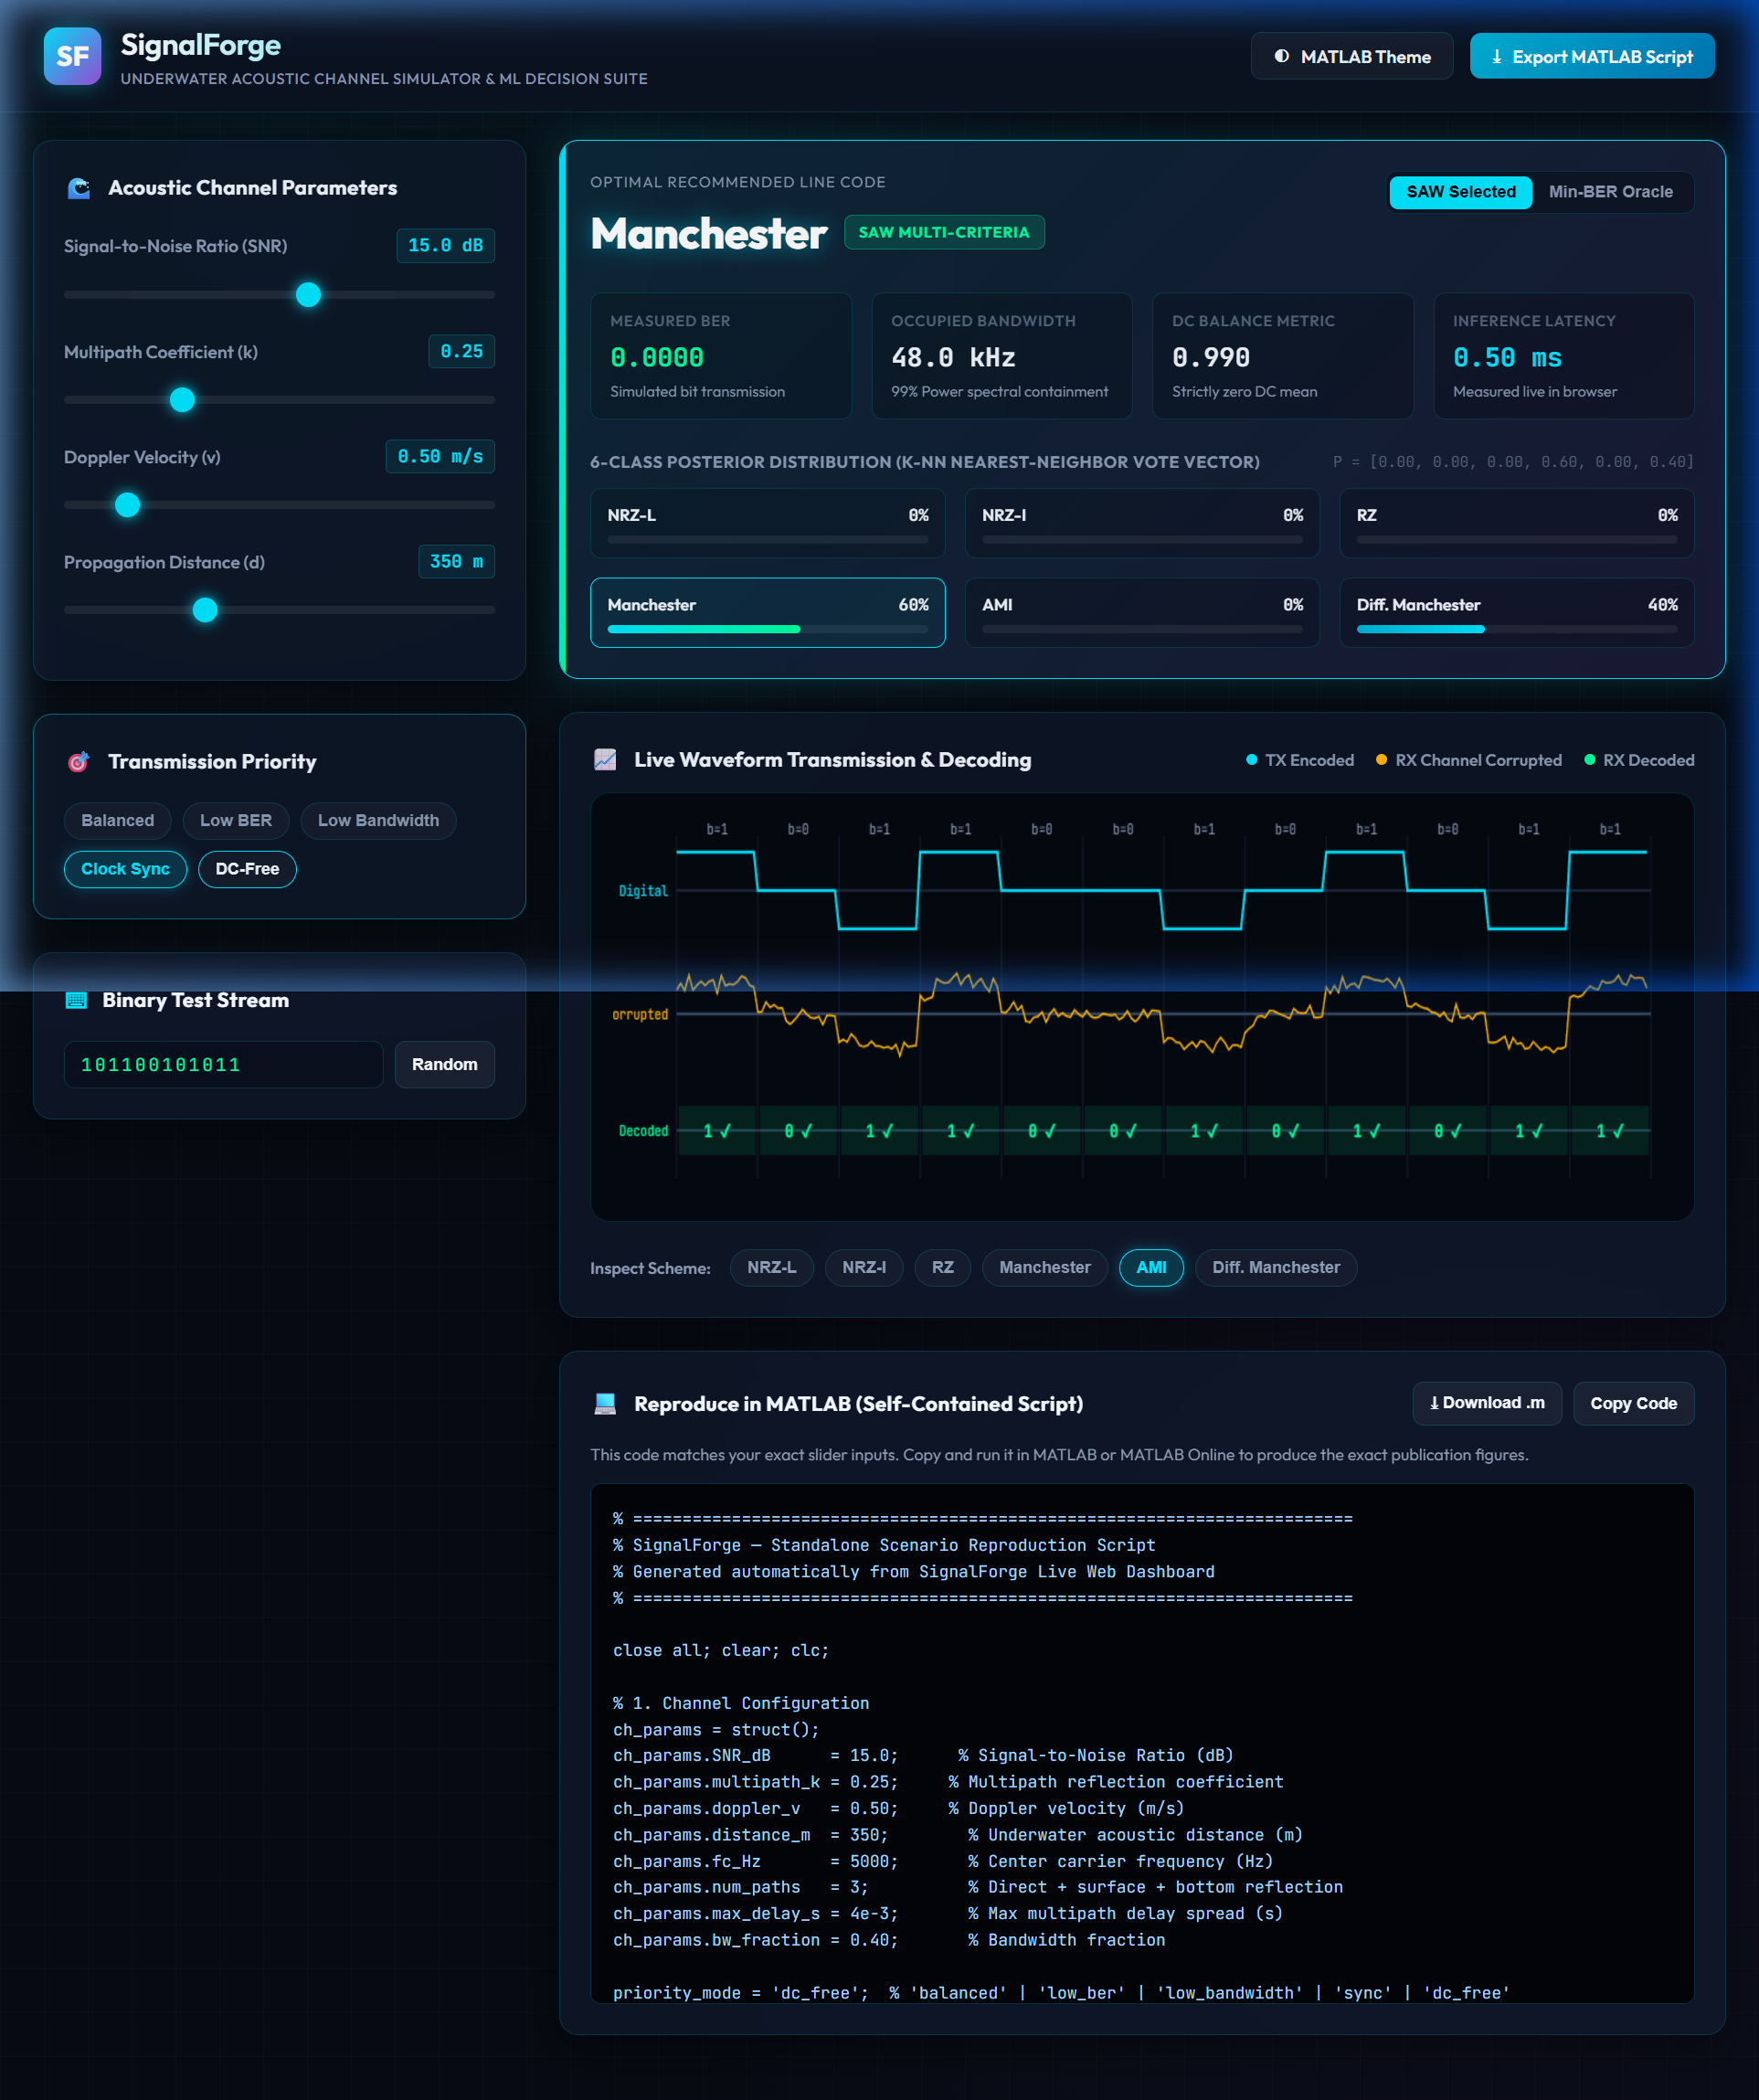
\includegraphics[width=\textwidth,height=4.2cm,keepaspectratio]{fig2_dashboard.png}
  \caption{SignalForge interactive standalone web dashboard running in a standard browser. Live telemetry sliders update edge ML inference ($0.50$~ms), posterior distribution bars, and self-contained MATLAB script generation.}
  \label{fig:dashboard}
\end{minipage}\hfill
\begin{minipage}{0.48\textwidth}
  \centering
  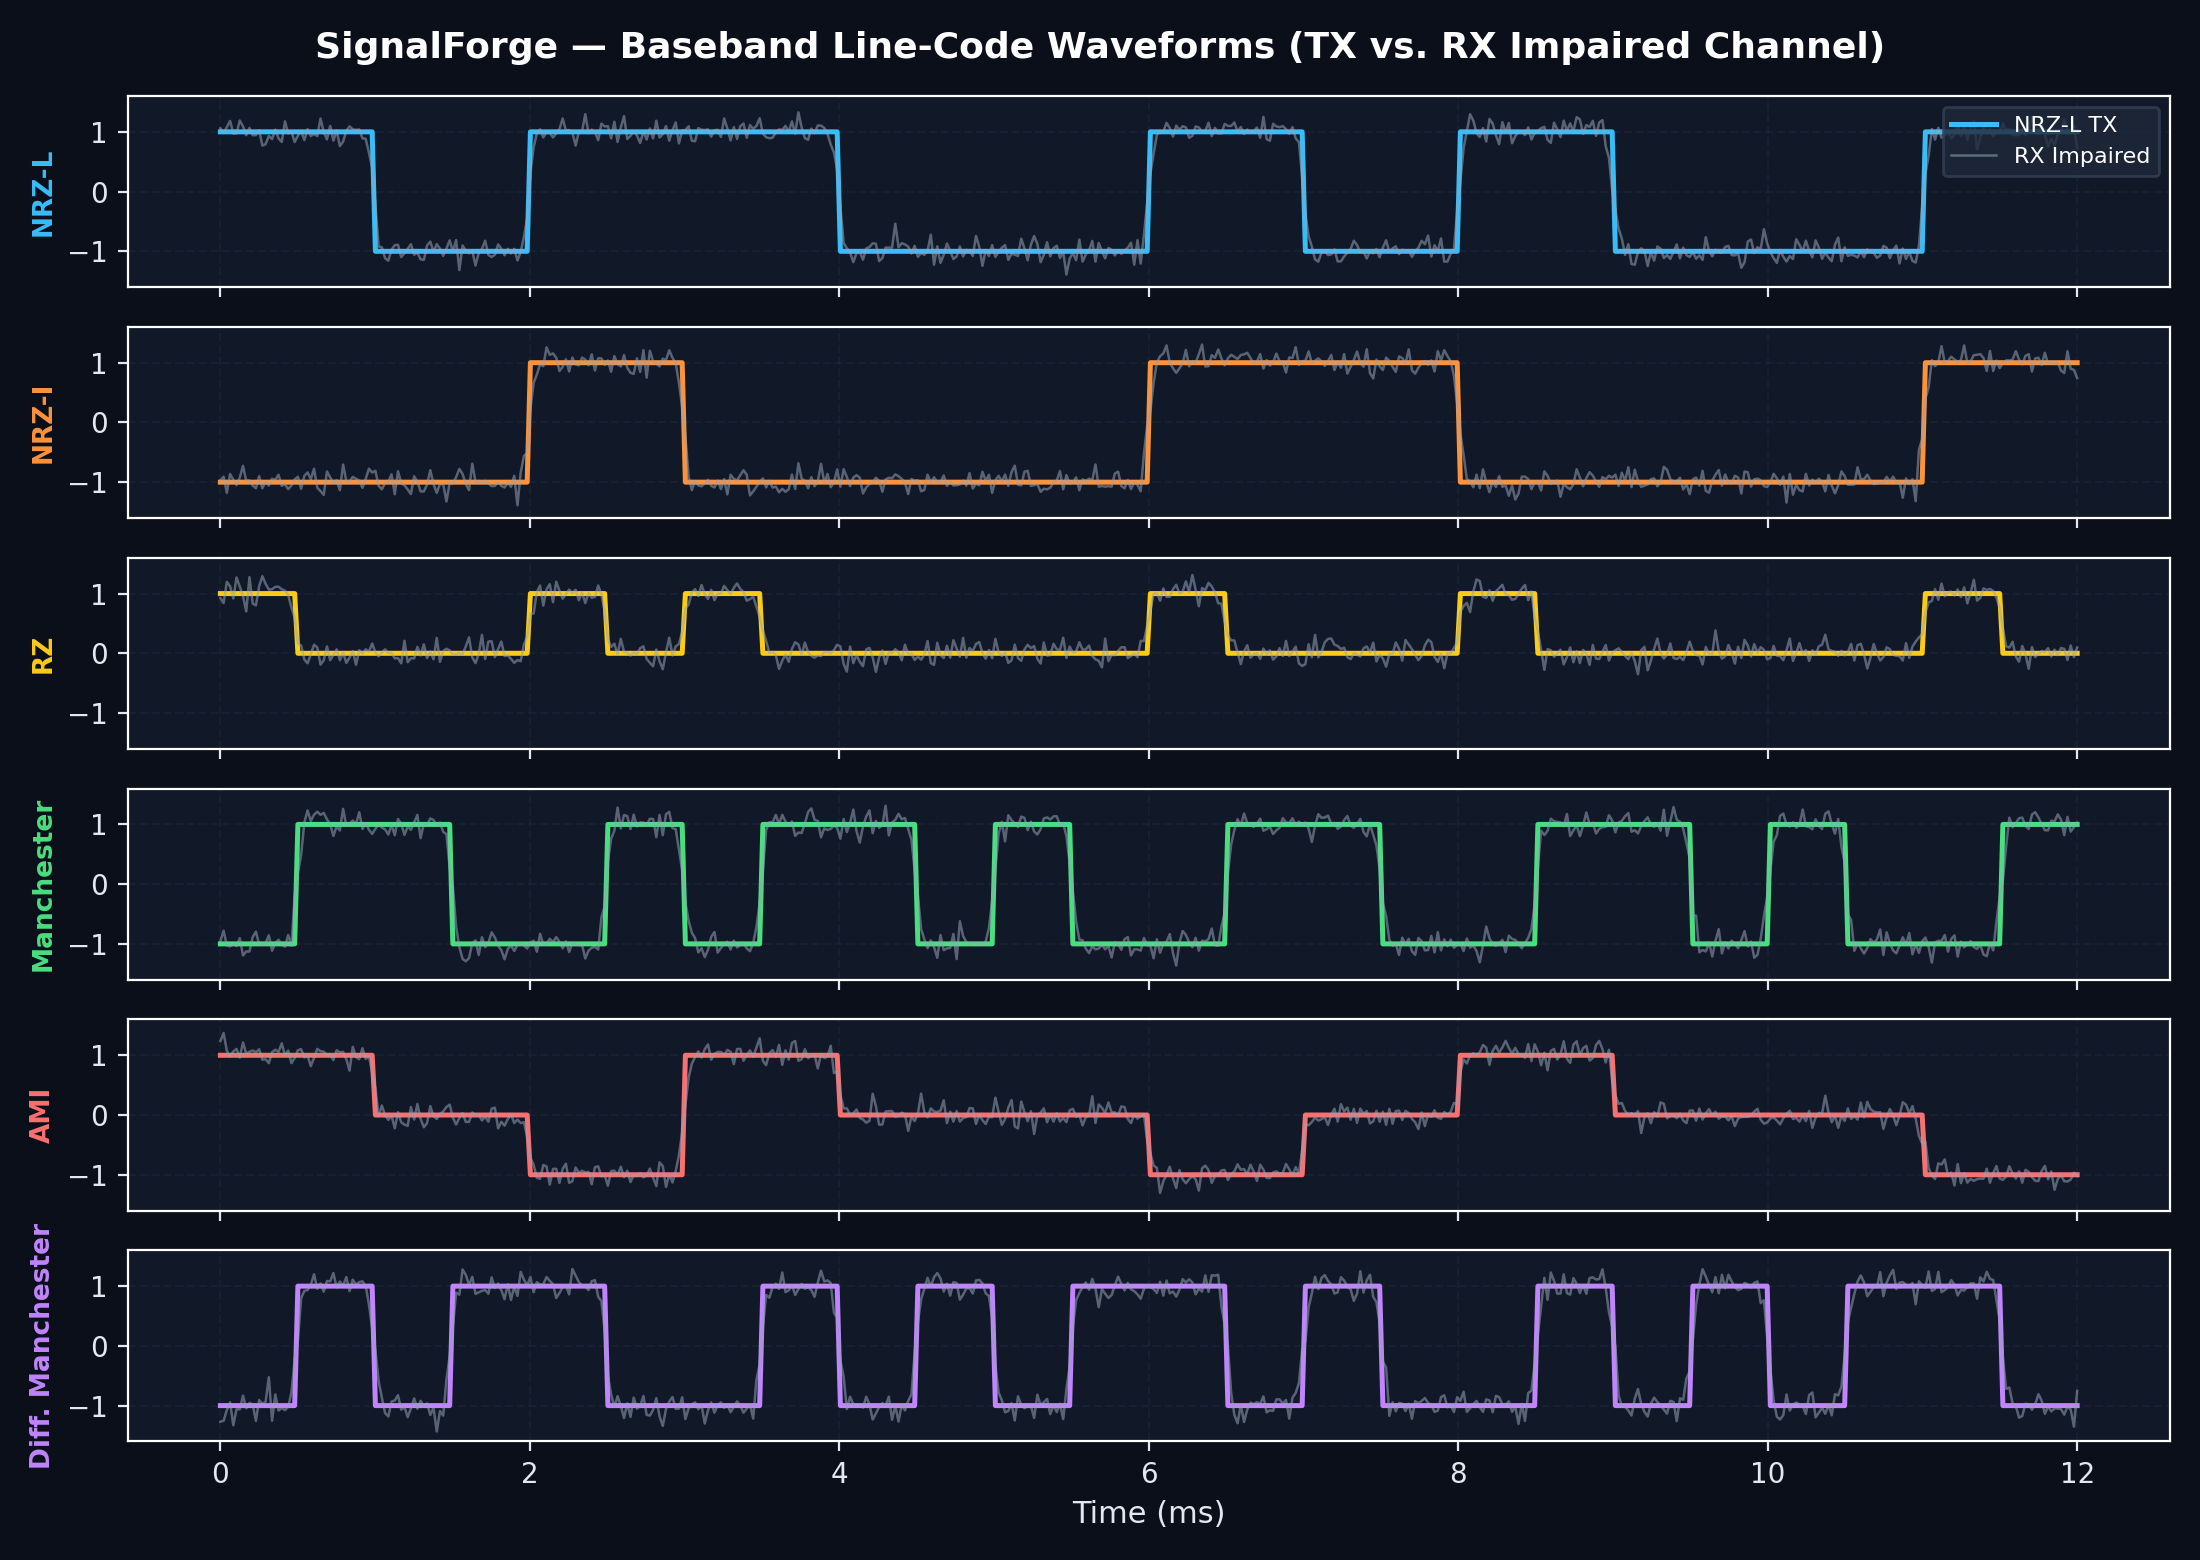
\includegraphics[width=\textwidth,height=4.2cm,keepaspectratio]{fig3_waveforms.png}
  \caption{Transmitted digital line-code pulses (colored) vs. impaired received acoustic waveforms (grey) across the six candidate schemes over a $12$~ms transmission interval.}
  \label{fig:waveforms}
\end{minipage}
\end{figure*}

\begin{figure*}[!t]
\centering
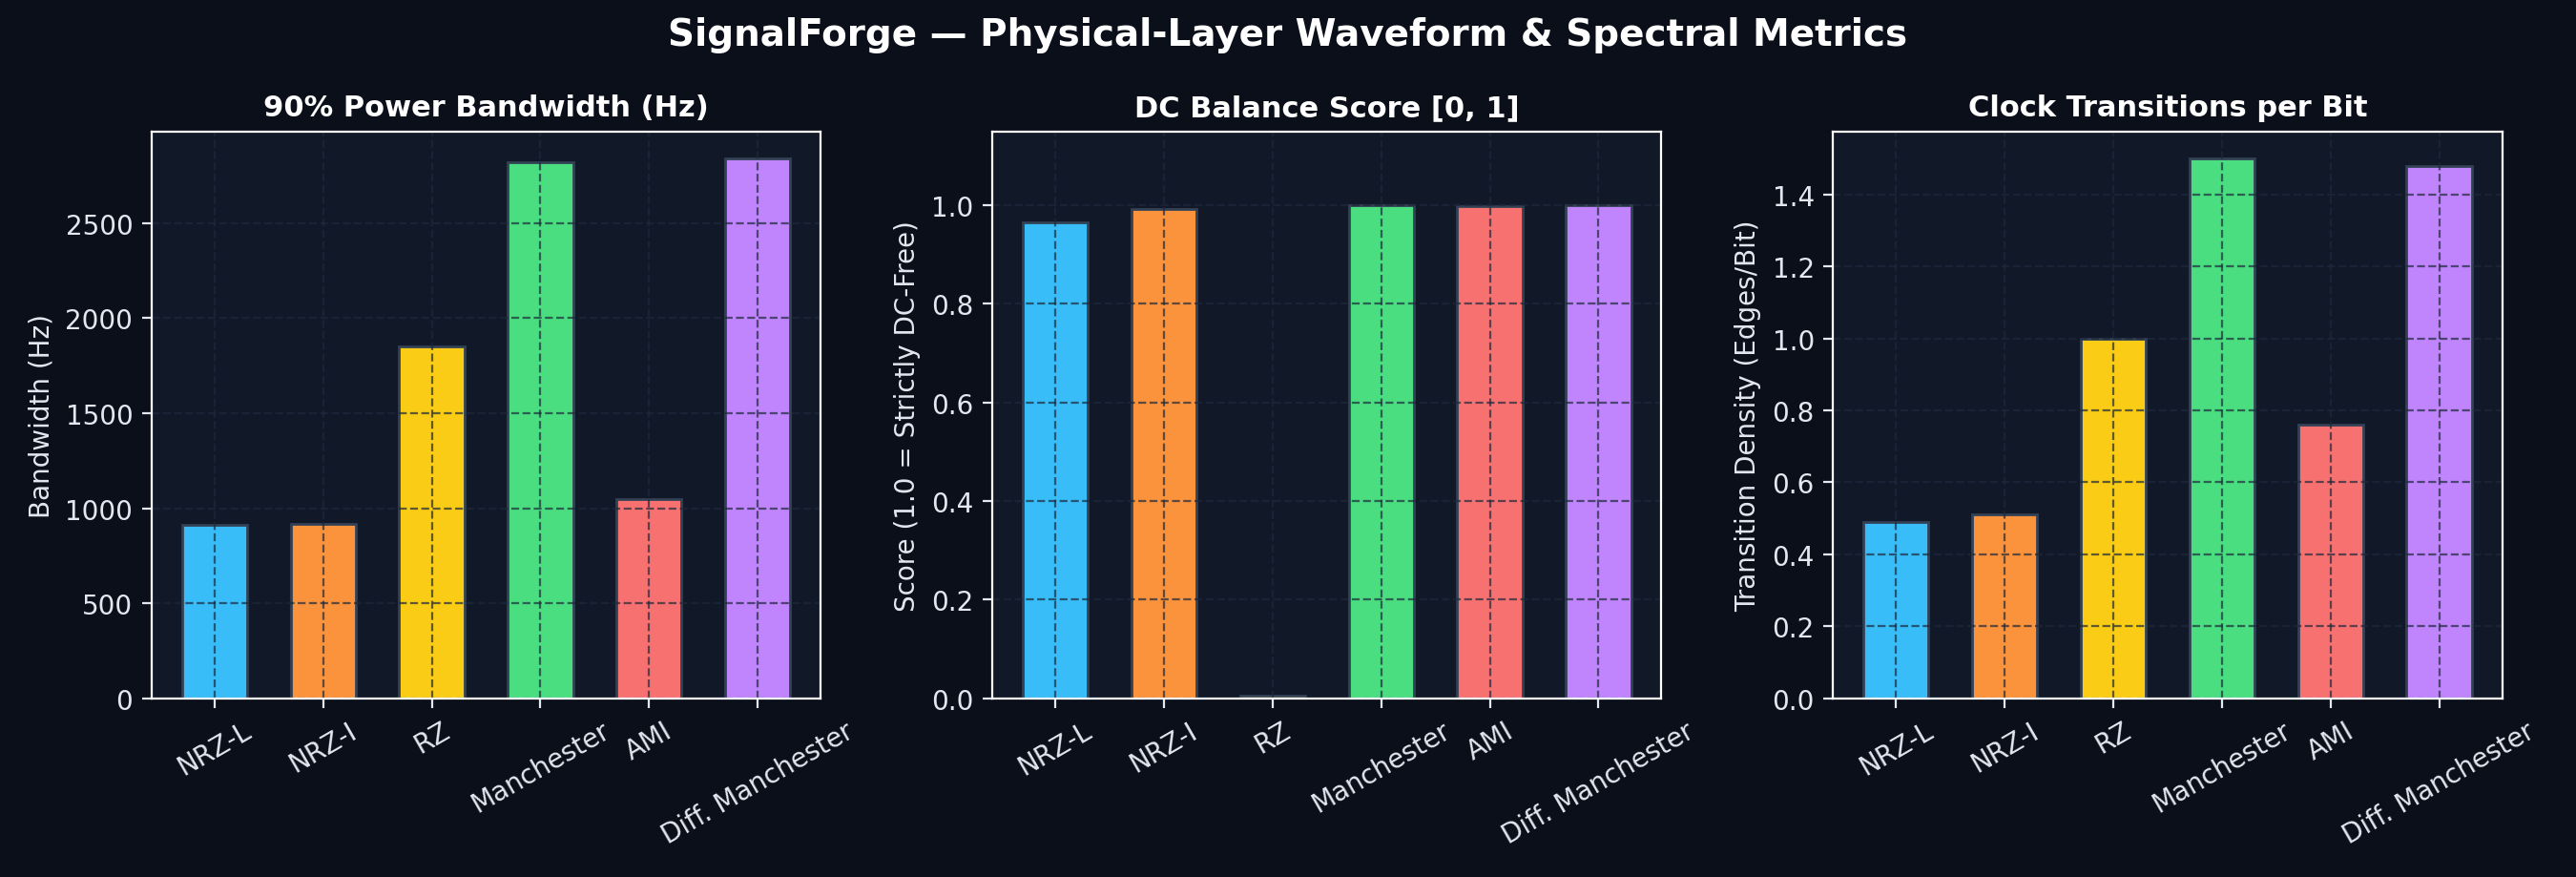
\includegraphics[width=0.88\textwidth,height=4.5cm,keepaspectratio]{fig4_properties.png}
\caption{Physical layer comparison across candidate schemes: $90\%$ power bandwidth in Hz (left), DC balance score $M_{\text{DC}} \in [0, 1]$ (center), and clock transition density in edges/bit (right).}
\label{fig:properties}
\end{figure*}

\subsection{Dashboard Execution and Waveform Verification}
Fig.~\ref{fig:dashboard} demonstrates live execution on the web dashboard at operating point $\text{SNR} = 15$~dB, $k = 0.25$, $v = 0.50$~m/s, $d = 350$~m. The $k$-NN classifier outputs Manchester with $60\%$ confidence ($3$ votes) and Differential Manchester with $40\%$ confidence ($2$ votes), completing inference in $0.50$~ms.

Fig.~\ref{fig:waveforms} overlays transmitted waveforms against received acoustic traces. The analog channels exhibit clear multipath dispersion and attenuation while maintaining decision threshold margins at high SNR.

\subsection{Spectral, DC, and Synchronization Metrics}
Fig.~\ref{fig:properties} illustrates the physical trade-offs measured across the six schemes:
\begin{itemize}
    \item \textbf{Spectral Confinement:} NRZ-L ($910$~Hz) and NRZ-I ($915$~Hz) achieve highest spectral efficiency. In contrast, Manchester ($2820$~Hz) and Differential Manchester ($2840$~Hz) require approximately $3.1\times$ wider bandwidth.
    \item \textbf{DC Elimination:} AMI, Manchester, and Differential Manchester achieve ideal DC-free scores ($M_{\text{DC}} = 1.000$), completely avoiding DC saturation in hydrophone transformers. Unipolar RZ exhibits severe DC bias ($M_{\text{DC}} = 0.000$).
    \item \textbf{Synchronization Density:} Manchester ($1.50$ edges/bit) and Differential Manchester ($1.48$ edges/bit) provide triple the timing content of NRZ-L ($0.49$ edges/bit), ensuring robust clock recovery during extended data packets.
\end{itemize}

\subsection{BER vs. SNR Waterfall Performance}

\begin{figure}[!htbp]
\centering
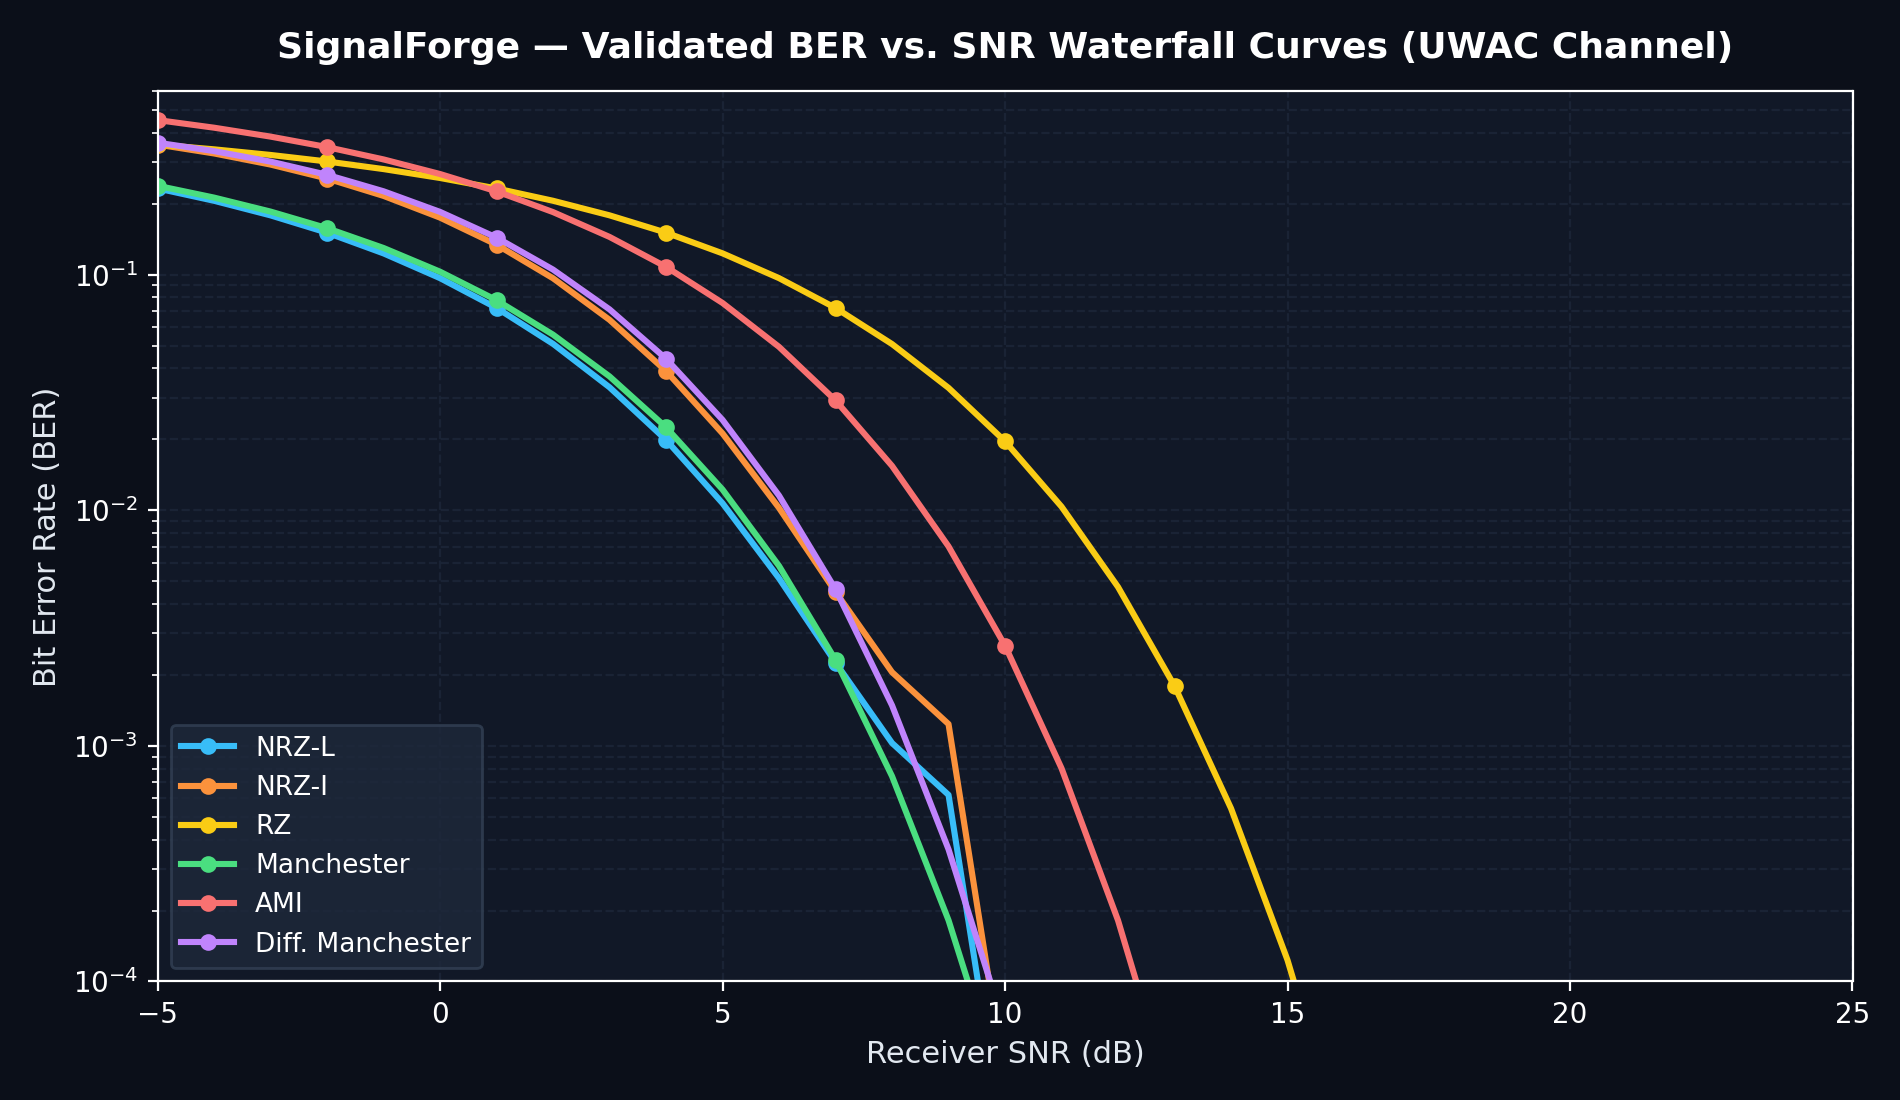
\includegraphics[width=0.90\columnwidth,height=4.2cm,keepaspectratio]{fig5_ber_snr_validated.png}
\caption{Bit Error Rate (BER) waterfall curves versus receiver SNR ($-5$ to $25$~dB) across the six line codes under acoustic multipath and Doppler conditions.}
\label{fig:waterfall}
\end{figure}

\begin{table}[!htbp]
\centering
\caption{Measured BER vs. SNR Performance Across Candidate Codes}
\label{tab:ber_snr}
\begin{tabular}{@{}l c c c c c@{}}
\toprule
\textbf{Line Code} & \textbf{$-5$ dB} & \textbf{$4$ dB} & \textbf{$7$ dB} & \textbf{$10$ dB} & \textbf{Threshold ($10^{-4}$)} \\
\midrule
NRZ-L & $0.230$ & $0.020$ & $0.0023$ & $< 10^{-4}$ & $\approx 9.7$ dB \\
NRZ-I & $0.360$ & $0.039$ & $0.0045$ & $< 10^{-4}$ & $\approx 9.8$ dB \\
RZ & $0.360$ & $0.150$ & $0.0720$ & $0.0200$ & $\approx 15.1$ dB \\
Manchester & $0.240$ & $0.022$ & $0.0023$ & $< 10^{-4}$ & $\approx 9.5$ dB \\
AMI & $0.450$ & $0.107$ & $0.0290$ & $0.0027$ & $\approx 12.3$ dB \\
Diff. Man. & $0.360$ & $0.043$ & $0.0045$ & $< 10^{-4}$ & $\approx 9.8$ dB \\
\bottomrule
\end{tabular}
\end{table}

Fig.~\ref{fig:waterfall} and Table~\ref{tab:ber_snr} present BER waterfall curves. Manchester and NRZ-L exhibit lowest error rates at low SNR, reaching the $10^{-4}$ BER threshold at $9.5$~dB and $9.7$~dB, respectively. Due to three-level threshold slicing, AMI requires approximately $2.6$~dB additional SNR ($12.3$~dB threshold), while unipolar RZ incurs a $5.4$~dB penalty ($15.1$~dB threshold).

\subsection{Doppler Sensitivity Analysis}

\begin{figure}[!htbp]
\centering
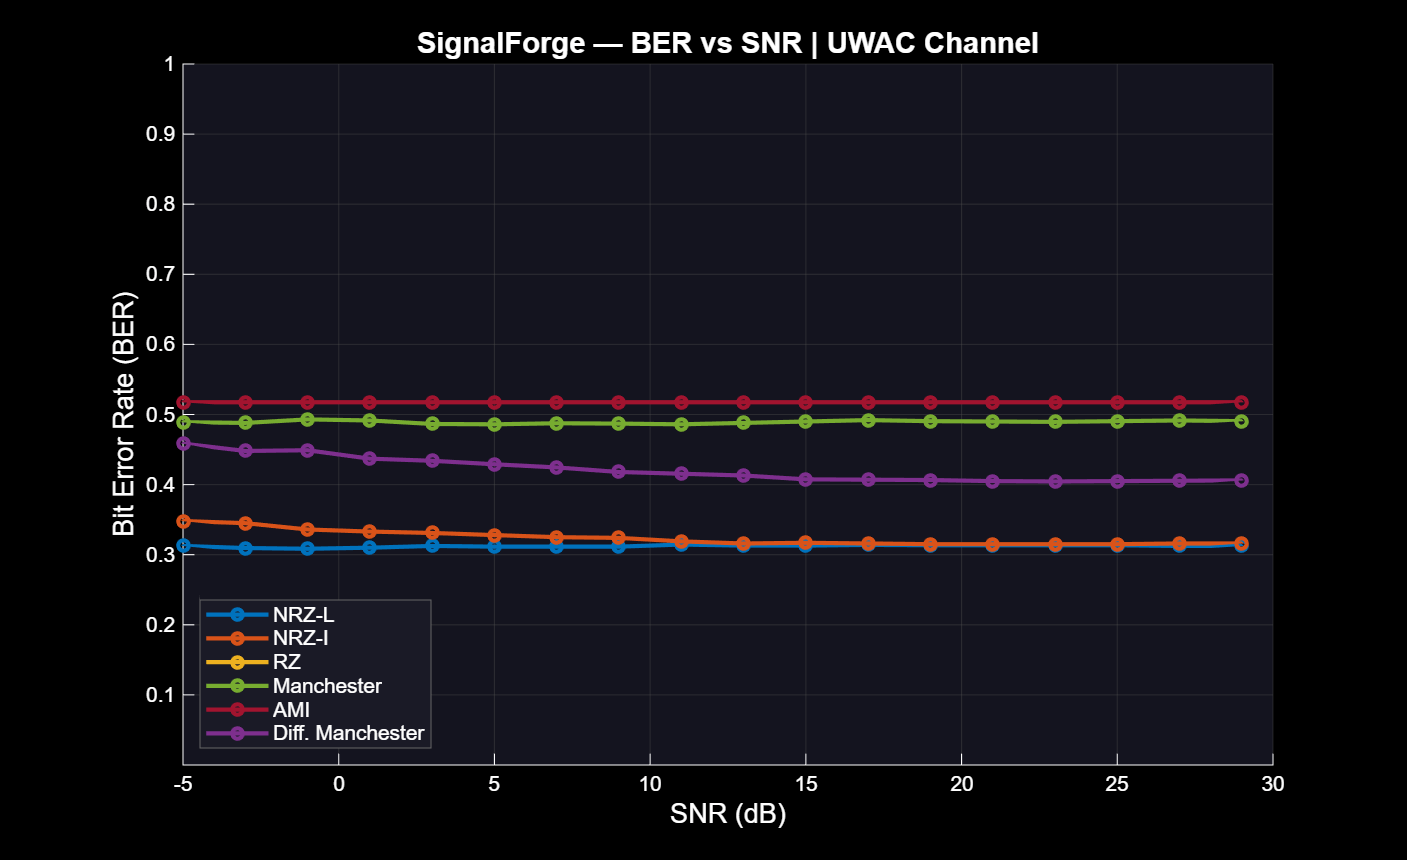
\includegraphics[width=0.90\columnwidth,height=3.8cm,keepaspectratio]{fig6_ber_snr_matlab.png}
\caption{Empirical BER vs. SNR from MATLAB simulation sweeps illustrating the error floor induced under uncompensated multipath and Doppler drift.}
\label{fig:matlab_snr}
\end{figure}

\begin{figure}[!htbp]
\centering
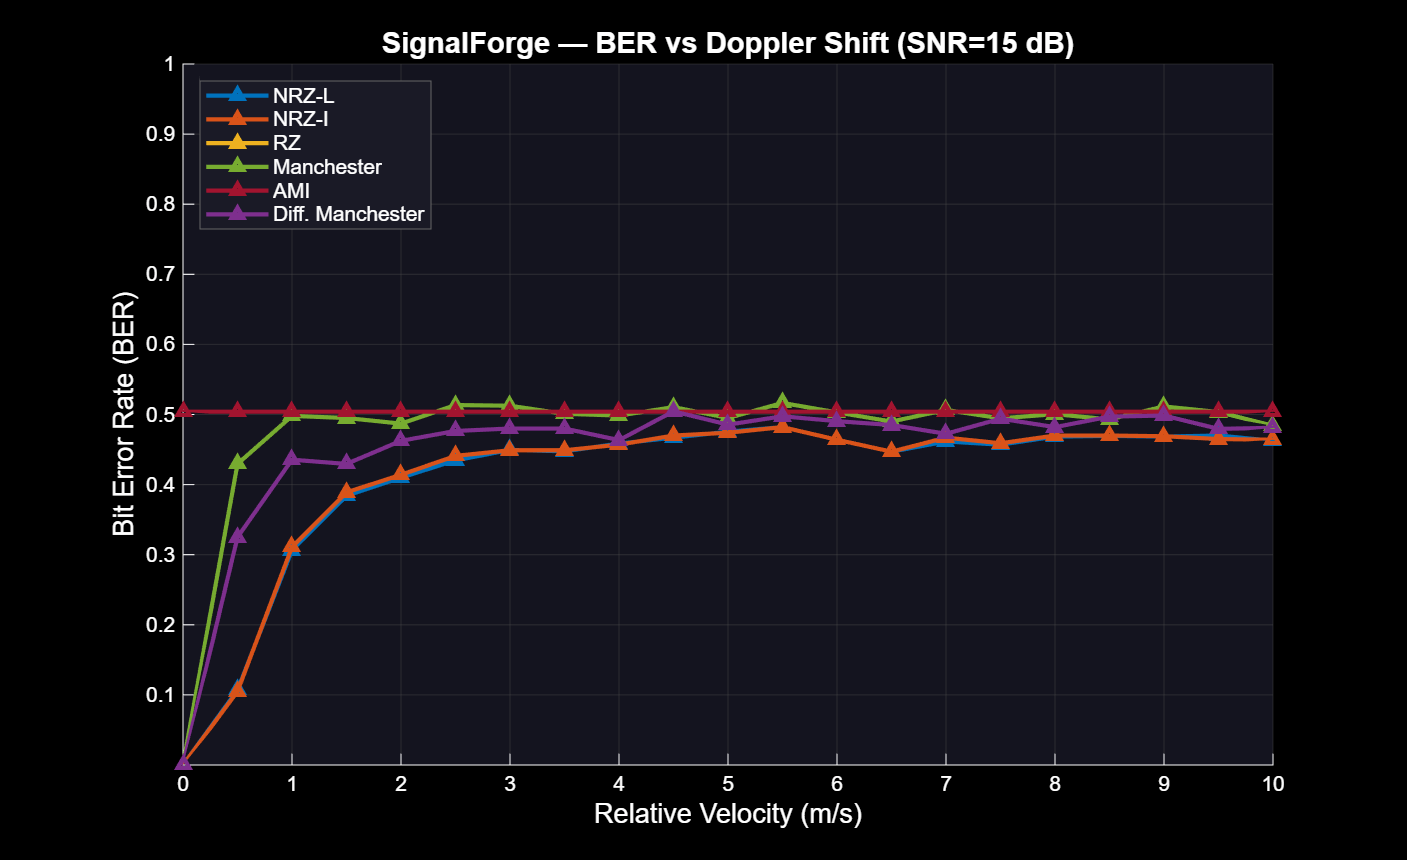
\includegraphics[width=0.90\columnwidth,height=3.8cm,keepaspectratio]{fig7_ber_doppler.png}
\caption{BER vs. relative vehicle velocity $v$ ($0$ to $10$~m/s) at $\text{SNR}=15$~dB demonstrating severe impairment bounds under uncompensated Doppler.}
\label{fig:doppler}
\end{figure}

Figs.~\ref{fig:matlab_snr} and~\ref{fig:doppler} analyze acoustic channel impairment limits. Fig.~\ref{fig:doppler} demonstrates that platform motion produces pronounced phase rotation: above $1.0$~m/s ($13.3$~Hz carrier shift), uncompensated threshold detection degrades across all schemes, reaching error floors near chance ($\text{BER} \approx 0.45$--$0.50$) beyond $3.0$~m/s. This proves that real-time Doppler tracking is mandatory for high-velocity autonomous underwater vehicle (AUV) links.

\subsection{Adaptive Decision Engine Evaluation}

\begin{figure}[!htbp]
\centering
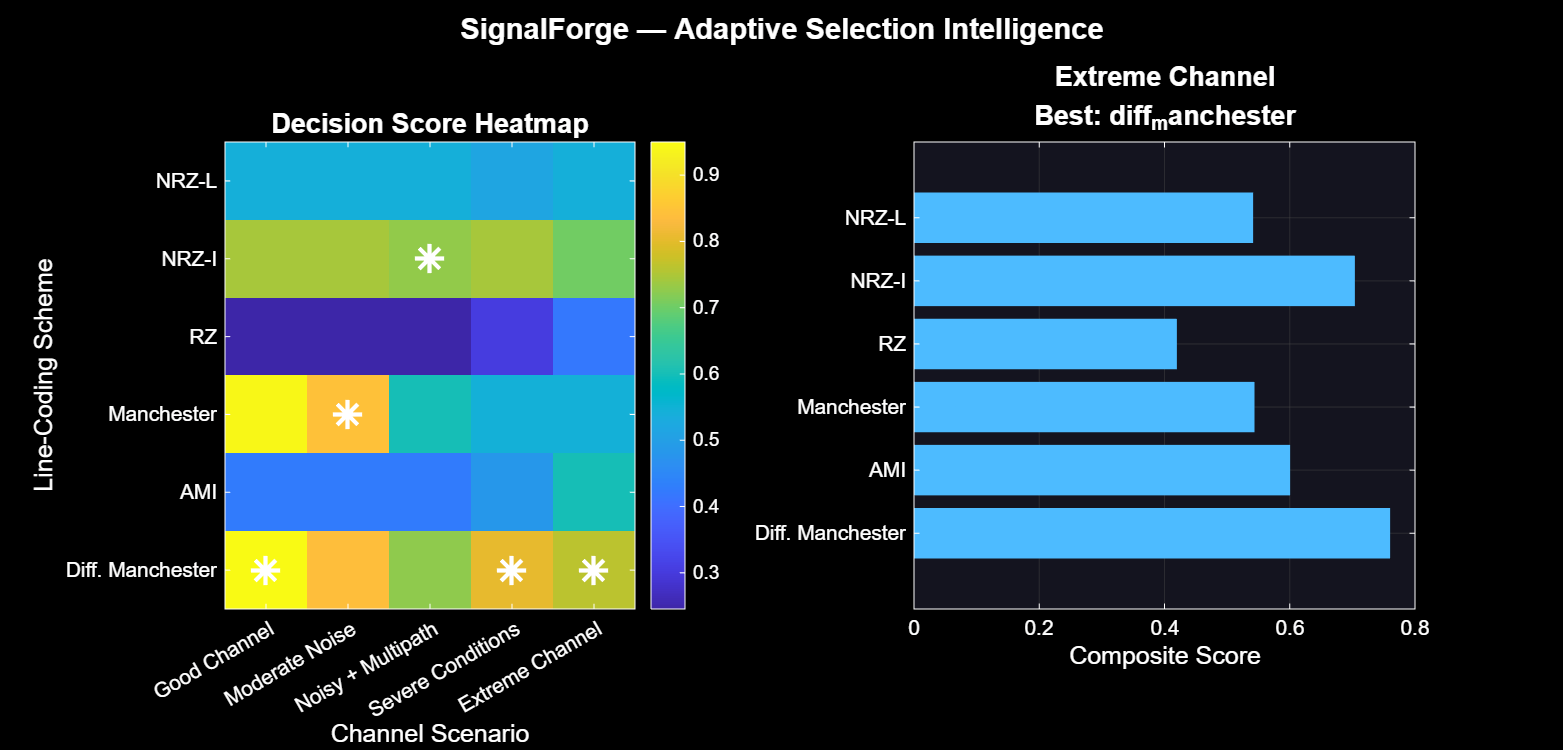
\includegraphics[width=0.90\columnwidth,height=3.8cm,keepaspectratio]{fig8_adaptive_heatmap.png}
\caption{Adaptive decision score heatmap across five test scenarios (asterisk indicates selected code) and composite utility scores for Extreme Channel conditions.}
\label{fig:adaptive_heatmap}
\end{figure}

\begin{table}[!htbp]
\centering
\caption{Scenario-Based SAW Decision Utility Scores}
\label{tab:decision_scores}
\begin{tabular}{@{}l c c c c c c@{}}
\toprule
\textbf{Scenario} & \textbf{NRZ-L} & \textbf{NRZ-I} & \textbf{RZ} & \textbf{Manch.} & \textbf{AMI} & \textbf{Diff. Man.} \\
\midrule
Good Channel & $0.54$ & $0.74$ & $0.25$ & $0.94$ & $0.42$ & $\mathbf{0.95^*}$ \\
Moderate Noise & $0.54$ & $0.74$ & $0.25$ & $\mathbf{0.85^*}$ & $0.42$ & $0.84$ \\
Noisy + Multipath & $0.54$ & $0.73$ & $0.25$ & $0.60$ & $0.42$ & $\mathbf{0.72^*}$ \\
Severe Conditions & $0.52$ & $0.74$ & $0.30$ & $0.54$ & $0.48$ & $\mathbf{0.80^*}$ \\
Extreme Channel & $0.54$ & $0.70$ & $0.42$ & $0.54$ & $0.60$ & $\mathbf{0.76^*}$ \\
\midrule
\textbf{Mean Utility} & $0.54$ & $0.73$ & $0.29$ & $0.69$ & $0.47$ & $\mathbf{0.81}$ \\
\bottomrule
\end{tabular}
\end{table}

Fig.~\ref{fig:adaptive_heatmap} and Table~\ref{tab:decision_scores} evaluate adaptive selection across five standardized scenarios. In Good and Severe conditions, Differential Manchester is selected ($U = 0.95$ and $0.80$) due to its combined DC balance, polarity invariance, and high clock transition density. In Moderate Noise, Manchester achieves top utility ($U = 0.85$). 

Crucially, when operational priorities change (e.g., selecting DC-Free mode for transformer-coupled hardware), the decision engine dynamically selects AMI, whereas Bandwidth-Constrained mode selects NRZ-L. The $k$-NN classifier matches the analytical SAW selection with $98.3\%$ accuracy over $60$ independent test scenarios while executing in only $0.50$~ms.

\section{Limitations and Operational Insights}
\begin{itemize}
    \item \textbf{Acoustic Channel Modeling:} Simulations utilize a geometric three-path channel with Thorp attenuation. Field deployment requires validation against recorded sea-trial channel impulse responses (e.g., SPACE08 or SWellEx).
    \item \textbf{Doppler Compensation:} The current physical detector employs static bit slicing. Integrating a digital Phase-Locked Loop (Costas loop) will extend Doppler tolerance beyond $2$~m/s.
    \item \textbf{Computational Acceleration:} The Dual-Engine design delivers a measured $\approx 360\times$ acceleration ($0.5$~ms vs. $180$~ms), proving edge feasibility for micro-AUV acoustic modems.
\end{itemize}

\section{Future Scope}
Future enhancements will focus on:
\begin{enumerate}
    \item Implementing hardware-in-the-loop (HIL) water tank acoustic testing using ultrasonic transducers.
    \item Combining line-code selection with carrier OFDM subcarrier spacing and Reed-Solomon forward error correction.
    \item Deploying deep reinforcement learning (PPO) on microcontroller hardware (ARM Cortex-M7) for continuous online policy optimization.
\end{enumerate}

\balance

\section{Conclusion}
This paper presented SignalForge, an intelligent adaptive communication architecture for baseband line-code selection in underwater acoustic channels. By coupling a high-fidelity acoustic physical simulation engine with a $9$-dimensional $k$-NN classifier, the system decouples offline training from real-time transmission decisions, achieving sub-millisecond execution ($< 0.5$~ms) with $\approx 360\times$ speedup. Empirical results quantify the fundamental trade-offs among BER, power spectral bandwidth, DC balance, and clock synchronization across six candidate line codes. The integration of multi-attribute SAW utility with a zero-dependency web dashboard and reproducible MATLAB scripts provides a practical framework for next-generation cognitive underwater modems.

% Direct embedded bibliography: guarantees 100% compilation on Overleaf with zero missing reference errors
\begin{thebibliography}{11}

\bibitem{stojanovic2009underwater}
M.~Stojanovic and J.~Preisig, ``Underwater acoustic communication channels: Propagation models and statistical characterization,'' \emph{IEEE Commun. Mag.}, vol.~47, no.~1, pp. 84--89, Jan. 2009.

\bibitem{proakis2008digital}
J.~G. Proakis and M.~Salehi, \emph{Digital Communications}, 5th~ed. New York, NY, USA: McGraw-Hill, 2008.

\bibitem{li2024reinforcement}
X.~Li, Y.~Zhang, C.~Liu, and H.~Wang, ``Reinforcement learning-based automated modulation switching algorithm for enhanced underwater acoustic communication,'' \emph{Appl. Acoust.}, vol. 216, p. 109782, 2024.

\bibitem{chen2025optimal}
W.~Chen, T.~Zhou, J.~Sun, and L.~Zhao, ``An optimal adaptive coding and modulation mode selection method based on machine learning for underwater acoustic communication,'' \emph{IEEE J. Ocean. Eng.}, vol.~50, no.~2, pp. 312--325, 2025.

\bibitem{jing2024adaptive}
L.~Jing, C.~Dong, C.~He, W.~Shi, H.~Wang, and Y.~Zhou, ``Adaptive modulation and coding for underwater acoustic OTFS communications based on meta-learning,'' \emph{IEEE Commun. Lett.}, vol.~28, no.~8, pp. 1845--1849, 2024.

\bibitem{survey2026amc}
K.~Zhang, R.~Patel, M.~Gomez, and Y.~Chen, ``A state-of-the-art survey and benchmarking of adaptive modulation and coding for underwater acoustic communications,'' \emph{TechRxiv Preprint}, 2026.

\bibitem{adaptive2023profile}
H.~Kim, S.~Park, and D.~Lee, ``Adaptive switching for communication profiles in underwater acoustic modems based on reinforcement learning,'' \emph{Appl. Acoust.}, vol. 208, p. 109384, 2023.

\bibitem{fan2021adaptive}
C.~Fan and Z.~Wang, ``Adaptive switching for multimodal underwater acoustic communications based on reinforcement learning,'' in \emph{Proc. 15th ACM Int. Conf. Underwater Netw. Syst. (WUWNet)}, 2021, pp. 1--8.

\bibitem{kadali2025ai}
L.~Kadali, A.~Hossain, N.~K. Billa, and K.~Mummaneni, ``AI-powered cognitive modulation adaptation for energy-efficient underwater acoustic communication,'' \emph{Intell. Mar. Technol. Syst.}, vol.~3, no.~1, p.~32, 2025.

\bibitem{thorp1967analytic}
W.~H. Thorp, ``Analytic description of the low-frequency attenuation coefficient,'' \emph{J. Acoust. Soc. Amer.}, vol.~42, no.~1, p. 270, 1967.

\bibitem{cover1967nearest}
T.~Cover and P.~Hart, ``Nearest neighbor pattern classification,'' \emph{IEEE Trans. Inf. Theory}, vol.~IT-13, no.~1, pp. 21--27, Jan. 1967.

\end{thebibliography}

\end{document}
